\chapter{Návrh designu}
Tato kapitola se zabývá návrhem designu stolní hry a~aplikace, která bude sloužit jako její součást. Jsou zde popsány požadavky na aplikaci, návrh grafického rozhraní a~návrh herních prvků.

\section{Požadavky na aplikaci}
Před samotným návrhem, bylo nutné stanovit požadavky, které by měla aplikace splňovat. Tyto požadavky byly stanoveny na základě analýzy stolních her \textit{Na vlnách neznáma}, \textit{Gloomhaven} a~\textit{Dungeons \& Dragons} a~na základě požadavků, které vyplynuly z~návrhu hry.

\subsection{Vzhled}
Vzhled aplikace by měl odrážet tématiku hry. Ta je situovaná do temného fantaskního světa s~RPG prvky. Samotná aplikace by tato témata měla reflektovat. Aby si hra uchovala tento temný nádech, tak bylo vybráno několik málo následujících barev, které se v~aplikaci vyskytnou. Základem designu ovládacích prvků budou odstíny tmavě šedé, které budou doplněny o~zelené prvky pro zvýraznění a~indikaci interaktivních prvků. Všechny tyto barvy budou v~kontrastu s~bílou barvou, která, společně se světlými odstíny šedé, bude použita pro texty a~popisky. Tímto způsobem bude vytvořen jednotný vzhled aplikace, který pomůže hráčům se v~ní lépe orientovat

Zážitek ze hry bude podporován tematickými obrázky, které hráčům pomohou lépe se do hry vcítit. Obrázky budou použity na pozadí herních stránek, ikonách postav a~nepřátel a~na kartách, které budou hráči používat. Tyto obrázky budou vygenerovány pomocí umělé inteligence, o~které se bude hovořit v~Kapitole \ref{sec:image_generation}.

Vzhled aplikace by měl být jednoduchý a~přehledný. Hráči by měli mít možnost snadno se na stránce orientovat a~mít přehled o~všech herních prvcích.

\subsection{Uživatelský zážitek}
Aby měli uživatelé ze hry co nejlepší zážitek, bylo rozhodnuto, že aplikace bude mít několik základních vlastností, které zlepší uživatelský zážitek.

\subsubsection*{Ovládání}
Ideální použití aplikace počítá s~tím, že ji hráči budou promítat na velký monitor, kde budou mít možnost vidět všechny herní prvky. Dále je podstatné, aby bylo ovládání jednoduché a~intuitivní. Z~těchto důvodů bude většina části aplikace, které souvisí se samotným průběhem hry ovladatelná pouze pomocí myši, aby bylo dosaženo co největšího komfortu pro hráče.

\subsubsection*{Responzivita}
Ze stejného důvodu, který je zmíněný výše, vyplývá, že aplikace by měla dobře sedět na velké monitory. Na to však nelze vždy spoléhat, jelikož někteří hráči nemají takovéto zařízení k~dispozici. Proto je nutné, aby byla aplikace responzivní a~byla schopna se přizpůsobit různým velikostem obrazovek, a~to včetně mobilních zařízení.

\subsubsection*{Čtení textů}
Jedním z~požadavků je také čtečka textů. Aplikace by měla být za pomoci umělé inteligence schopna číst texty nahlas. Toto má řadu výhod, jako třeba dostupnost pro hráče, kteří mají problémy se čtením. Zároveň to může být také zajímavým prvkem, který by mohl zlepšit imerzi a~tím také celkový zážitek ze hry.

\subsubsection*{Perzistence dat}
Aplikace si udrží aktuální data i~po obnovení stránky. To znamená, že bude schopna ukládat data do databáze průběžně a~zobrazovat je hráčům i~po obnovení stránky. Tímto způsobem budou mít hráči možnost pokračovat v~dané části hry i~v~případě, že ji z~jakéhokoliv důvodu nebyli schopni dokončit či v~případě, že jsou nuceni stránku obnovit.

\subsection{Funkcionalita}
Aplikace bude sloužit jako nástroj pro ukládání hráčských dat a~pro správu herního světa. Hráči budou mít možnost vytvářet postavy, které budou moci upravovat a~vylepšovat. Postavy se budou moci účastnit dobrodružných bojových střetnutí, které budou záviset na hráči určených kampaních. Jednotlivá střetnutí budou mít vlastní mapu představující hrací plochu a~budou obsahovat nepřátele, kteří budou mít své vlastní schopnosti a~statistiky. Všechny tyto informace budou uloženy v~databázi a~hráčům přístupny právě přes webové rozhraní.

Následující funkcionality vyplývají z~vlastního návrhu, který vzešel z~analýzy některých titulů a~zkušeností nabytých hraním stolních her:

\subsubsection*{Přihlášení}
Jeden z~funkčních požadavků, která bude aplikace splňovat, je možnost přihlášení. Hráči dostanou přiřazené unikátní licenční číslo a~heslo, které jim umožní se do aplikace přihlásit. Přihlášení bude pro hru nutné, jelikož se tak budou ukládat data o~postavách a~kampaních, které hráči vytvoří.

\subsubsection*{Vytváření dobrodružství}\label{sec:adventure}
Dobrodružstvím se rozumí kombinace postav a~herního příběhu (neboli kampaně), který určuje průběh a~cíl hry. Ke každému účtu bude možno vytvořit takovýchto dobrodružství několik a~hráči budou schopni mezi nimi vybírat. Při jejich tvorbě budou hráči vyzváni k~zadání názvu a~popisu a~k~výběru kampaně. Ta bude pomocí API získána z~databáze a~bude obsahovat informace o~lokacích, které mohou být ve hře navštíveny, nepřátelích, kteří se v~nich mohou vyskytovat a~o~odměnách, které hráči mohou získat.

\subsubsection*{Vytváření postav}
Podobně jako u~dobrodružství, aplikace bude povolovat vytváření hráčských postav. Ty se budou skládat ze dvou základních částí. Ty jsou rasa a~povolání, jejichž výběr každé postavě udá unikátní schopnosti a~statistiky. Postavy budou mít možnost se v~průběhu hry vyvíjet a~získávat schopnosti nové.

\subsubsection*{Bojové střetnutí}
Bojová střetnutí budou základním a~hlavním prvkem hry. Bude se jednat o~souboj mezi hráči a~nepřáteli, který bude probíhat na fyzické herní ploše. Konfigurace této herní plochy bude zobrazena v~aplikaci a~bude záviset na konkrétním dobrodružství. Aplikace bude mít v~tomto případě za cíl držet v~paměti aktuální stav hry, informace o~postavách a~nepřátelích a~zobrazovat je hráčům v~reálném čase. Dále bude aplikace zobrazovat informace o~akcích, které mohou nepřátelé provádět a~bude tímto způsobem hráčům sdělovat, jak se má hra vyvíjet.

\subsubsection*{Správa předmětů}
Tato funkcionalita byla nakonec odsunut pro budoucí rozšíření hry. Aplikace bude umožňovat hráčům dostávat odměny za splnění úkolů a~za porážku nepřátel. Tyto odměny budou mimo jiné v~podobě předmětů s~různými účinky, které budou moci být použity v~boji. Zároveň budou mít hráči možnost tyto předměty nakupovat za herní měnu, kterou budou taktéž získávat za splnění úkolů. Hráči je budou moci přiřazovat k~postavám a~tím si zpřístupnit jejich účinky.

\section{Využití umělé inteligence}
Umělou inteligenci je možné v~tomto projektu využít hned v~několika případech. Jedním z~nich je generování obrázků, které budou použity v~grafickém rozhraní aplikace. Dále je možné využít umělou inteligenci pro předčítání textů. V~této kapitole si popíšeme, jak by mohla být umělá inteligence využita v~těchto dvou případech.

\subsection{Generování obrázků}\label{sec:image_generation}
Existuje velká řada nástrojů, které umožňují generování obrázků pomocí umělé inteligence. Většina z~nich využívá neuronové sítě, které byly natrénovány na velkém množství dat. Tyto sítě jsou pak schopny generovat obrázky na základě těch, které byly pro trénování použity. Využití takovýchto nástrojů většinou obnáší jakousi sadu slov, jakožto vstupní parametr (těmto slovům se běžně říká prompty), na základě které je obrázek vygenerován. V~našem případě půjde například o~popis vzhledu nepřátel, které by hráči mohli potkat v~průběhu hry.

Při výběru technologie, která bude pro tento účel použita, bylo vyzkoušeno několik nástrojů. Mezi ně patří například lokálně nainstalovaný model \textit{Stable Diffusion} \cite{stability_ai}. Jedná se o~open-source model, kterému lze nahrát jednu z~mnoha volně dostupných datových sad a~upravit tak styl výsledných obrázků. Tento nástroj se však ukázal jako nepoužitelný, kvůli jeho náročnosti na lokální stroj a~kvůli jeho nekonzistentním výsledkům. Dále byl vyzkoušen nástroj \textit{Midjourney} \cite*{midjourney}, kterému se bude věnovat následující sekce.

Obě tyto technologie využívají difuzní modely. Jsou to generativní modely, což znamená, že jsou použity ke generování podobných dat, na kterých byly trénovány. Jsou učeny tak, že ničí trénovací data pomocí postupného přidávání gaussovského šumu a~následně se snaží tato data rekonstruovat pomocí inverzního procesu. Při generování nových dat si model nejprve pomocí náhodně zvoleného čísla vytvoří náhodný šum a~následně ho pomocí inverzního procesu převede na obrázek.

\subsubsection*{Midjourney}
Tento model je dostupný online a~jeho využívání je v~současné době podmíněno předplatným. Byl však schopen generovat obrázky, které byly velmi kvalitní a~téměř dokonale odpovídaly našim požadavkům. Díky tomu byl tento nástroj vybrán pro použití v~našem projektu.

Pro generování obrázků bylo nutné se zaregistrovat na oficiální stránce \textit{Midjourney} a~zajistit předplatné. Stránka následně poskytne přístup k~API, se kterým lze komunikovat přes sociální platformu Discord. Pomocí příkazu \texttt{/imagine} je možné modelu poslat sadu promptů, které se pro generování použijí, jak lze vidět na Obrázku \ref{fig:mj_prompts}. Výsledný obrázek je následně zaslán zpět uživateli. Ten se může rozhodnout, zda je výsledek uspokojivý či nikoliv a~popřípadě provádět různé úpravy.

\begin{figure}[H]
    \centering
    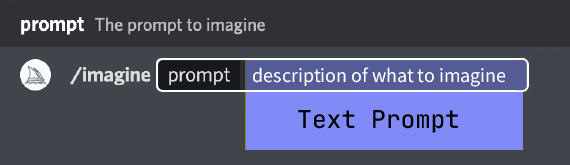
\includegraphics[width=0.475\textwidth]{resources/figures/midjourney_prompts.png}
    \caption{Příkaz pro generování obrázku pomocí \textit{Midjourney} \cite{midjourney}}
    \label{fig:mj_prompts}
\end{figure}

Tento proces je však také možné obrátit. Modelu je možné poslat obrázek ve formě odkazu. Ten je následně zanalyzován a~na základě něj je vygenerován několik textových popisů, které by měly daný vstup vystihnout. Tento způsob je velmi užitečný v~případech, kdy chce uživatel použít pouze určité části či kvality daného obrázku jako předlohu pro generování dalších. \textit{Midjourney} je také schopno přímo ze vstupních obrázků vygenerovat obrázky nové. V~tomto případě však bere model v~potaz celý obrázek, což může být v~některých případech nežádoucí.

Mimo promptů lze modelu předat i~parametry, které dále alterují výstup. Ty se označují dvěma pomlčkami před samotným parametrem. Velmi užitečným se jeví být parametr \texttt{{-}{-}no} pro negativní prompty. To jsou takové prompty, které modelu říkají, co by obrázek neměl obsahovat. Dále lze však využít parametry jako \texttt{{-}{-}style}, který mění styl obrázku či \texttt{{-}{-}cref}, díky kterému lze do výsledku přidat konkrétní postavu v~různých kompozicích. Tímto způsobem je možné přesněji specifikovat a~ovlivnit požadovaný výstup. Celý vstupní řádek je možné vidět na Obrázku \ref{fig:mj_prompts_params}.

\begin{figure}[H]
    \centering
    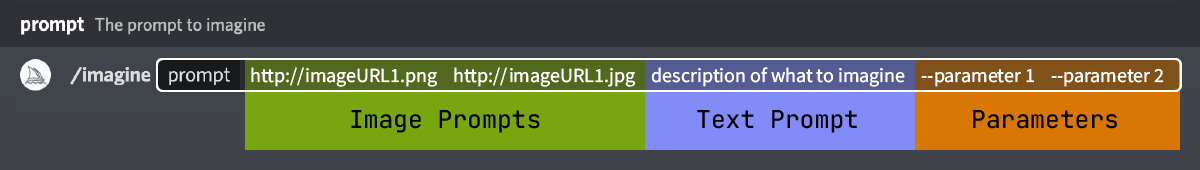
\includegraphics[width=1\textwidth]{resources/figures/midjourney_prompts_params.png}
    \caption{Příkaz pro generování obrázku s~parametry pomocí \textit{Midjourney} \cite{midjourney}}
    \label{fig:mj_prompts_params}
\end{figure}

\subsection{Předčítání textu}
Pro tento účel by bylo možné využít některý z~text-to-speach nástrojů, jejichž zdrojové kódy jsou dostupné online. Tyto nástroje jsou schopny přečíst text, který je jim zadán a~pomocí algoritmů a~neuronových sítí generovat věrnou napodobeninu lidského hlasu. Výhodou těchto nástrojů je, že jsou schopny přečíst texty v~mnoha jazycích a~že jsou schopny generovat hlas, který zní velmi přirozeně.

Z~časových důvodů bylo rozhodnuto, že tato funkcionalita nebude do aplikace implementována, avšak by mohla být v~budoucnu přidána jako rozšíření.

\section{Návrh fyzických komponent}
Návrh této stolní hry počítá s~několika fyzickými komponentami, které budou mít hráči k~dispozici. Mezi tyto komponenty patří herní plocha, figurky postav a~nepřátel, karty s~hráčskými akcemi, karty s~předměty a~upravená dvacetistěnná kostka. Jejich návrh zle vidět na Obrázku \ref{fig:physical_components}.

\subsection{Herní plocha}
Herní plocha pro každou z~lokací bude tvořena z~dílů, které bude možno skládat k~sobě. Propojovat je budou speciální dílky, které budou představovat dveře mezi jednotlivými místnostmi. Díly budou mít na sobě vyobrazena hexagonová pole, které budou reprezentovat možnosti, kam hráč bude moci v~průběhu hry pohnout svou postavu. Na těchto políčkách budou umístěny figurky postav a~nepřátel a~také tokeny pastí a~překážek.

Samotná plocha bude vytištěna na speciální papír, který bude přilepen na materiál vyrobený z~lisovaného papíru. Tento způsob se běžně v~herním průmyslu používá. Potisk desky bude vygenerován pomocí umělé inteligence a~vytištěn ve vysokém rozlišení. Mezi další materiály, které byly zvažovány, patří například plastové desky, které by byly odolnější a~mohly by být použity i~jako magnetické. Tyto desky by však byly mnohem dražší a~jejich výroba by byla náročnější, proto byly pro tento projekt zavrženy. Bylo by však možné tuto možnost použít například pro prémiové vydání hry.

\subsection{Kostka}
Bylo rozhodnuto, že pro tuto hru bude použit jeden druh kostky. Bude se jednat o~dvacetistěnnou kostku, která bude upravena s~ohledem na potřeby hry. Na ní budou vyobrazeny symboly nacházející se v~Tabulce \ref{tab:dice_symbols}. Kostka bude vyrobena z~odlitého polymeru. Tento materiál byl zvolen, jelikož je odolný a~zároveň dostatečně lehký.

\begin{table}[H]
    \centering
    \begin{tabular}{*{21}{c}}
        \toprule
        \multicolumn{1}{c|}{\textbf{Symbol}} & MISS & -4 & -4 & -3 & -3 & -2 & -2 & -1 & -1 & 0 & 0 & 1 & 1 & 2 & 2 & 3 & 3 & 4 & 4 & CRIT \\
        \bottomrule
    \end{tabular}
    \caption{Symboly na dvacetistěnné kostce}
    \label{tab:dice_symbols}
\end{table}

\subsection{Figurky}
Zatímco rozhodnutí o~herní ploše bylo poměrně jednoduché, rozhodnutí o~figurkách bylo mnohem složitější. Figurky by měly být dostatečně odlišné, aby hráči neměli problém je od sebe rozeznat. Bylo zvažováno několik možností výroby figur, od 2D tisku na karton, přes 3D tisk, až po vstřikování plastů. Každá z~těchto možností má své výhody a~nevýhody, o~kterých budou pojednávat následující sekce.

\subsubsection*{3D tisk}
3D tisk by umožnil vytvořit figurky, které by byly téměř identické s~těmi, které byly vygenerovány pomocí umělé inteligence. Existuje několik variant tisku. FDM tisk by byl nejlevnější, avšak nejméně kvalitní. SLA tisk by byl naopak dostatečně kvalitní, avšak mnohem dražší. Další nevýhodou 3D tisku je jeho časová náročnost. Zároveň je nutné mít k~dispozici 3D model, který by byl pro tisk použit. Z~důvodu nedostupnosti nástrojů, které by dokázaly správně a~kvalitně převést 2D obrázek na 3D objekt, by bylo nutné tento model vytvořit ručně. Tento způsob by byl tedy velmi náročný na čas a~bylo by třeba zajistit, aby byl model dostatečně kvalitní pro samotný tisk.

V~omezené míře jsme však tento způsob použili pro vytvoření prototypu hracího plánu. Ty byly vytvořeny pomocí FDM tisku, a~jelikož se jednalo pouze o~zkušební verzi, byly přiměřeně kvalitní pro účely testování. Pro finální verzi to však nebylo dostatečné.

\subsubsection*{Vstřikování plastů}
Vstřikování plastů je technologie, která je za použití forem schopna vytvořit velké množství identických plastových dílů ve velmi krátkém čase. V~závislosti na kvalitě formy a~typu zvoleného materiálu mohou být výsledné produkty velice detailní a~odolné. Tato technologie by byla ideální pro výrobu figur, avšak je velmi nákladná a~náročná na výrobu forem.

\subsubsection*{2D tisk}
Figurky by byly vytištěny na karton a~následně vystřiženy. Tento způsob by byl nejlevnější a~nejrychlejší, ale nejméně kvalitní. Figurky by byly náchylné k~poškození a~mohly by být snadno poničeny.

\subsubsection*{Zvolené řešení}
Z~důvodu časové náročnosti a~nákladů bylo rozhodnuto ve prospěch 2D tisku. Figurky budou opatřeny plastovým stojánkem pro stabilitu a~zároveň budou použity různé barvy pro rozlišení hráčů a~nepřátel. Jedno z~předešlých řešení by však mohlo být použito pro prémiové vydání hry.

\subsection{Karty}
Budou barevně rozděleny podle jednotlivých ras a~povolání, kterým budou náležet. Zároveň na nich budou vyobrazeny texty a~obrázky, které budou reprezentovat jednotlivé akce. Karty budou vytvořeny z~odolného papíru a~budou opatřeny ochrannou vrstvou, která zamezí jejich poškození. Bylo rozhodnuto o~standardní velikosti karet, která je 63x88 mm.

\begin{figure}[H]
    \centering
    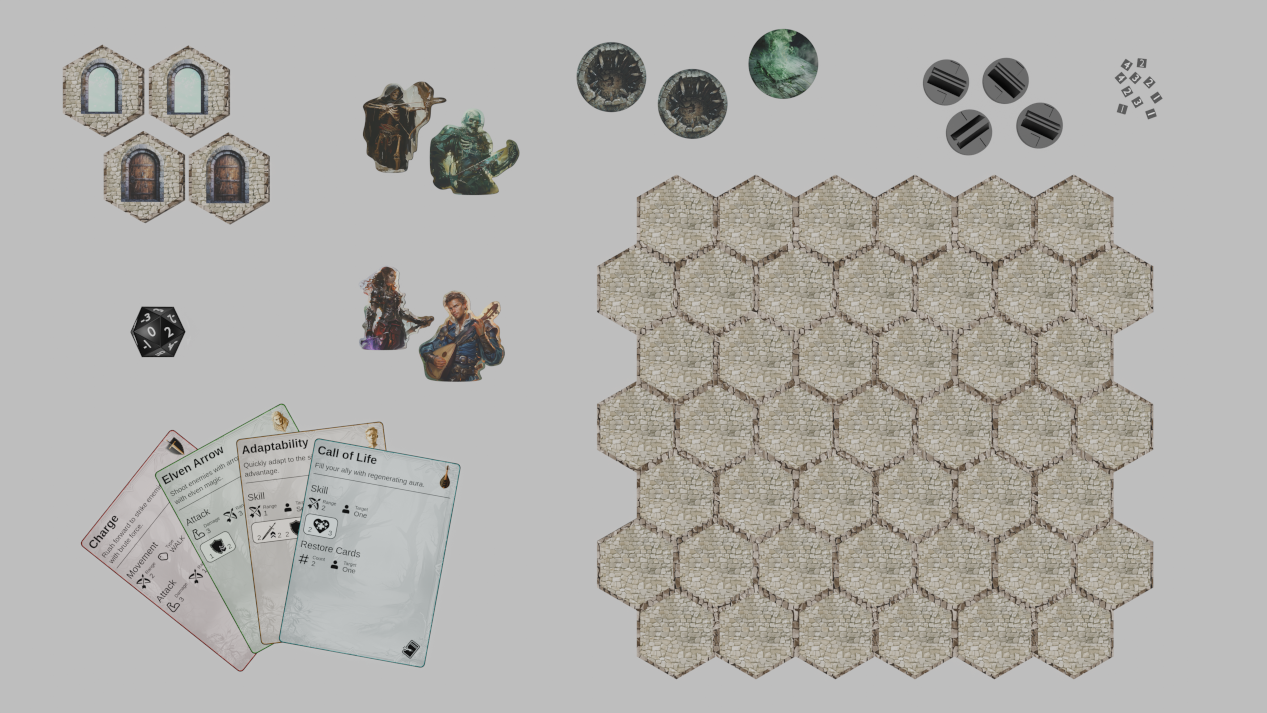
\includegraphics[width=0.9\textwidth]{resources/figures/components.png}
    \caption{Návrh fyzických komponent}
    \label{fig:physical_components}
\end{figure}

\section{Volba technologií pro vývoj aplikace}
Zprvopočátku jsem vytvořil prototyp GUI v~čistém HTML a~CSS, abych věděl, jak bude samotný produkt zhruba vypadat. Poté jsem svou pozornost obrátil na výběr technologií, které budu pro vývoj GUI používat.

\subsection{Frameworky}
Frameworky jsou nástroje, které usnadňují vývoj webových aplikací tím, že poskytují hotové komponenty, knihovny a~nástroje, které urychlují a~zjednodušují vývoj. Každý z~nich má své výhody a~nevýhody a~je vhodný pro jiné typy aplikací. Výběr správného frameworku závisí na požadavcích aplikace, na zkušenostech vývojáře a~na jeho preferencích. V~následujících odstavcích se budu věnovat třem populárním frameworkům pro tvorbu webových aplikací -- \textit{React}, \textit{Angular} a~\textit{Svelte}.

\subsubsection*{React}
\textit{React} je jednou z~nejpopulárnějších moderních platforem pro tvorbu webových aplikací. Je to open-source JavaScript knihovna vyvinutá a~udržovaná společností \textit{Meta} (bývalý \textit{Facebook}). Používá deklarativní programovací paradigma, což znamená, že vývojář specifikuje, jak by měl výsledek vypadat, bez toho, aby musel explicitně popsat, jak daného výsledku dosáhnout. Zároveň je založen na komponentovém přístupu -- celý kód je rozdělen do menších celků zvaných komponenty, což je kombinace JS a~HTML, které jsou modulární a~znovupoužitelné. Díky jeho schopnosti aktualizovat jednotlivé komponenty se nejčastěji používá pro vývoj jednostránkových webových aplikací. \textit{React} je známý svou komunitou a~ekosystémem, který je kolem něj postavený. Díky tomu je možné najít spoustu předpřipravených komponent a~knihoven, které urychlí vývoj aplikace. Zároveň má však poměrně strmou křivku učení, což z~něj dělá nepřívětivou volbu pro začátečníky.

\textit{React} využívá virtuální DOM, který zajišťuje rychlejší a~efektivnější vykreslování změn. Při změně v~komponentě se nevykreslí celá stránka, ale pouze upravená část. Tím se značně zrychlí vykreslování a~zároveň sníží nároky na výkon. \cite{react, what_react_is_and_why_it_matters,angular_vs_react}

\subsubsection*{Angular}
\textit{Angular} je další z~vysoce populárních frameworků pro vývoj UI. Opět se jedná o~open-source platformu, nyní však vyvinutou a~udržovanou společností \textit{Google}. \textit{Angular} je založen na jazyce TypeScript a~stejně jako \textit{React} využívá komponentového přístupu a~deklarativního programovacího paradigmatu. Jeho hlavní význam spočívá ve vytváření rozsáhlých dynamických webových aplikací. Na rozdíl od \textit{Reactu} se jedná o~plnohodnotný framework, který používá reálný DOM. Samotný framework je robustní a~bezpečný, což z~něj dělá ideální volbu pro vývoj aplikací, které pracují s~citlivými daty. Na druhou stranu je však poměrně složitý a~náročný na výkon, což je pro menší aplikace nevhodné. \cite{what_is_angular,angular_vs_react}

\subsubsection*{Svelte}
\textit{Svelte} je moderní framework pro tvorbu webových aplikací. Jedná se o~open-source software vyvinutý Richem Harrisem. Svelte se od ostatních frameworků liší tím, že se jeho kód při buildu převede na čistý optimalizovaný JavaScript. Tím se výsledná aplikace značně zrychlí a~zároveň se sníží nároky na výkon na straně uživatele. Svelte také nabízí velmi jednoduchý a~přívětivý způsob psaní kódu, který vývoj aplikace urychlí. Dokáže také pracovat s~TypeScript soubory bez nutnosti jejich předešlé kompilace, což výsledný kód dělá mnohem bezpečnějším a~přehlednějším. \cite{svelte_and_why_you_should_consider_it,svelte}

\subsubsection*{Srovnání}
Vzhledem k~tomu, že projekt obnáší vytvoření GUI pro hybridní stolní hru, která nebude nijak extrémně rozsáhlá, a~zároveň bude potřebovat co největší rychlost a~efektivitu, jsem nakonec zvolil framework \textit{Svelte}. Ten nabízí všechny potřebné funkce a~zároveň je velmi rychlý a~efektivní. Jeho jednoduchost by také měla přispět k~rychlejšímu vývoji bez dalších větších problémů.

\subsection{Knihovny UI}
Dále jsem se rozhodl používat CSS a~JS knihovny, které dokáží ušetřit práci s~designem a~responzivitou a~tím zrychlit vývoj aplikace.

\subsubsection*{Bootstrap}
\textit{Bootstrap} je jeden z~nejpopulárnějších nástrojů pro vytváření responzivních webových stránek. Je to open-source nástroj, který byl původně vyvinut pro sociální platformu \textit{Twitter} (nyní známou jako \textit{X}). Nabízí spoustu předpřipravených komponent, které velmi usnadní vývoj a~zároveň zlepší vzhled aplikace. Mimo to dává vývojáři možnost využít některé z~tříd, které dokáží nastylovat téměř jakýkoliv HRML element, kterému jsou přiřazeny. \textit{Bootstrap} je také velmi dobře zdokumentovaný a~má velkou komunitu uživatelů, takže je poměrně snadné najít řešení k~případným problémům. \cite{bootstrap,what_is_bootstrap}

\subsubsection*{Tailwind CSS}
\textit{Tailwind CSS} je další nástroj pro tvorbu responzivních webových stránek. Na rozdíl od \textit{Bootstrapu} je však známý svou flexibilitou a~možnostmi přizpůsobení. Je založen na konceptu utility-first, což znamená, že primárním cílem tohoto nástroje je užitek, s~čím se váže jednoduchost. Vývojáři mohou využít jednotlivé třídy, jenž \textit{Tailwind CSS} nabízí. Každá z~nich přidá pouze jeden určitý styl k~elementu a~dodává tak vývojáři možnost je mezi sebou kombinovat dle libosti. Tímto způsobem je možné vytvořit téměř jakýkoliv design, který si vývojář přeje. Opět se jedná o~velmi dobře zdokumentovaný nástroj s~také poměrně velkou komunitou. \cite{tailwind_css}

\subsubsection*{Svelte Material UI}
Jako jediný ze zde zmíněných, není tento nástroj agnostický a~je určen pouze pro framework \textit{Svelte}. \textit{Svelte Material UI} je knihovna komponentů, které jsou inspirovány vzhledem \textit{Material Design} od společnosti \textit{Google}. Tato knihovna je velmi užitečná pro vývojáře, kteří chtějí vytvořit aplikaci, která bude mít moderní a~čistý design. Díky faktu, že je určena přímo pro \textit{Svelte} je její použití opravdu jednoduché. Nevýhodou je, že není zdaleka tak rozsáhlá jako předešlé možnosti. \cite{svelte_material_ui}

\subsubsection*{Srovnání}
Po zvážení všech možností jsem se rozhodl pro knihovnu \textit{Bootstrap}. \textit{Svelte Material UI} přináší příliš ostrý a~strohý vzhled, který by pro tuto aplikaci nebyl vhodný. Bootstrap jsem nakonec vybral převážně z~preferenčních důvodů. Jsem s~ní dobře obeznámený a~vím, jak s~ní pracovat. Zároveň jsem si jist, že mi poskytne všechny potřebné komponenty a~nástroje, které budu pro vývoj aplikace potřebovat.

\subsection{Další knihovny}
Pro vývoj jsem se rozhodl použít několik dalších knihoven, které přidávají různé předpřipravené komponenty a~funkce. Toto mi umožnilo využít již existující řešení a~já se tak mohl zaměřit na samotný vývoj aplikace.

\subsubsection*{Notiflix}
\textit{Notiflix} je knihovna, která umožňuje vytvářet přehledné notifikace a~jednoduché načítací animace. Toto není to jediné, co tato knihovna nabízí, ale pro tento projekt byly využity pouze tyto funkcionality. \textit{Notiflix} je velmi jednoduchý a~přívětivý nástroj, který je velmi snadno použitelný a~zároveň nabízí spoustu možností pro úpravu vzhledu. \cite{notiflix}

\subsubsection*{Simplebar}
Tato knihovna přidá pouze jednoduchý scrollbar, který je mnohem přívětivější než ten, který používá většina prohlížečů. Tento scrollbar je menší a~diskrétnější, což zlepšuje celkový vzhled aplikace. \textit{Simplebar} je také velmi jednoduchý na použití a~není třeba žádného složitého nastavení. \cite{simplebar}

\subsection{Použité jazyky}
Hlavními jazyky pro vývoj webových aplikací jsou HTML, CSS a~JavaScript. Pro tento projekt jsem se rozhodl použít TypeScript, což je nadmnožina JavaScriptu, která přidává statické typování a~další funkce, které zvyšují bezpečnost a~přehlednost kódu. TypeScript je velmi populární mezi vývojáři a~Svelte framework ho plně podporuje.